\documentclass[10pt]{article}

\usepackage{amsmath}
\usepackage{graphicx}
\usepackage{clrscode3e}
\usepackage{caption}
\usepackage{floatrow}

\title{Design and analysis of algorithms}
\date{2019-12-1}
\author{Akshay Rajesh}

\begin{document}

\maketitle
\pagenumbering{gobble}

\newpage
\tableofcontents
\pagenumbering{gobble}

\newpage
\pagenumbering{arabic}

\section{Problem description}
Given a 2n-node undirected graph G(V,E); positive integer $k \leq G.E$ . Can the nodes of G be partitioned into 2 disjoint sets U and W each of size n and such that the total number of distinct edges in G.E that connect a node u in U to a node w in W is at most k?
\\
\\
The problem described above is the decision version of the well-known MINIMUM BISECTION PROBLEM. So let us call our problem K-BISECTION problem. A brief overview of MINIMUM BISECTION PROBLEM is given below.
\\
\\
\textbf{MINIMUM BISECTION PROBLEM}
\\\\
The MINIMUM BISECTION PROBLEM is a well-known NP-hard problem, which is intended to partition the vertices of a given graph into two equal halves so as to minimize the cost where cost is defined as the number of edges with two ends in 2 different halves. MINIMUM BISECTION was shown to be NP-hard by Garey, Johnson and Stockmeyer\cite{minbisectioncompleteness}.

\section{Problem formulation}
\textbf{K-BISECTION  PROBLEM }
\\\\
INPUT : $<G,k>$, where G is a graph encoding and k is a positive integer.\\\\
OUTPUT : YES, if $<G,k> \in L$\\
	     \hspace*{50pt} NO, otherwise \\\\
where language L is defined as follows, \\
L = \{$<G,k> | |G.V|=2n$ ,and G.V can be partitioned into U and V such that $U \cap V = \O$ and  $U \cup V= G.V$ and number of edges $(x,y) \in G.E$ such that $x \in U$ and $y \in V$ is at most $k$  \}.

\section{Solving MINIMUM BISECTION PROBLEM \\
using K-BISECTION as a subroutine}
Let ML be a deterministic Turing machine that determines if an encoded input $<G,k>$ belongs to language L or not. We use this machine to build a machine MBP which finds the min cost bisection of the input graph. The construction of this machine is shown in the figure below.

\begin{figure}[h!]
    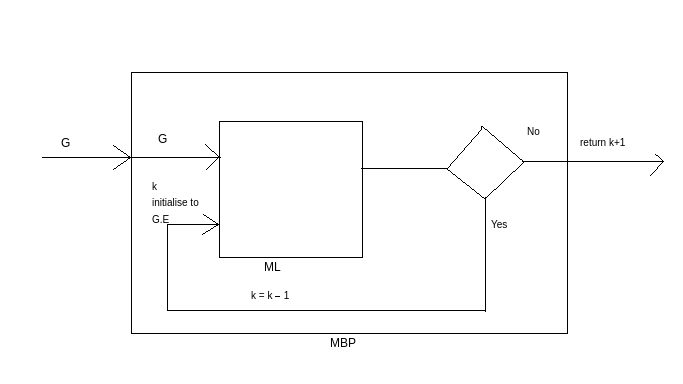
\includegraphics[width=\linewidth]{MBP.png}
    \caption{Machine to find min cost bisection}
    \label{fig:MBP}
\end{figure}

\section{Proof that K-BISECTION is NP-Complete}
To prove that the given problem is NP-Complete ,we have to show that it is both NP and NP-Hard.
\subsection{Proof that K-BISECTION is NP}
To prove that the problem is NP, we give a polynomial time verification algorithm for a certificate to the problem. We have as the certificate an encoding of  graph G , two sets of vertices V1 and V2 and a positive integer k. The algorithm is as follows


\begin{codebox}
\Procname{$\proc{Verify}(G,V1,V2,k)$}

\li \If $(|V1| \neq |V2|)$
     \Then
\li     \Return $\const{FALSE}$
     \End
\li \If $(V1 \cup V2 \neq G.V) \lor (V1 \cap V2 \neq \O)$
    \Then
\li     \Return $\const{FALSE}$
    \End
\li $\id{count} \gets 0$
\li \For $\forall u \in  \attrib{V1}$  \Do
\li      \For $\forall v \in  \attrib{V2}$ \Do  
\li         \If $(u,v) \in G.E$ \Then   
\li              $count \gets count + 1$
            \End
        \End
    \End
\li\If $count \leq k$ \Then   
\li         \Return $\const{TRUE}$
     \End
\li\Return $\const{FALSE}$      
\end{codebox}

\subsection{Proof that K-BISECTION is NP-Hard.}

To prove that this problem is NP-Hard, we give a reduction from K-CUT problem ,the decision version of MAX-CUT problem, which is already proved to be NP-Hard.

\subsubsection{MAX-CUT PROBLEM}
The MAX-CUT problem asks us to find a subset S of the vertex set of the given graph such that the number of edges between S and the complementary subset is as large as possible.

\subsubsection{K-CUT PROBLEM}
The K-CUT problem takes as input a graph G and a positive integer k and determines whether G contains a cut of size at most k or not.\\
K-CUT = \{$<G,k> |$ Graph G has a cut of size at most k\}.\\
\\

\subsubsection{Reduction from K-CUT to K-BISECTION}
Let the input to K-CUT problem be $<G,k>$ where G is a graph and k is a positive integer.

\begin{itemize}
\item Add $|G.V|$ isolated vertices to G to yield G’.
\item G’  now has $2 × |G.V |$ vertices.
\item As the newly added vertices have no edges, moving them around contributes nothing to the cut.
\item Every cut $(S, V-S)$ of G can be made into a bisection by appropriately allocating the new nodes between S and V - S.
\item Hence each cut of G can be made a cut of G’ of the same size, and vice versa.	
\item So the presence of a k-bisection in G’ implies the presence of a k-cut in G.
\end{itemize}

\begin{figure}[h!]
    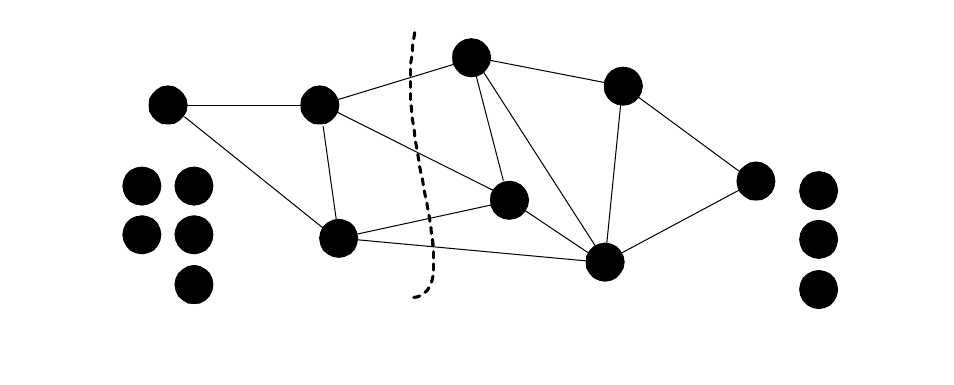
\includegraphics[width=\linewidth]{g_dash.png}
    \caption{Graph G'}
    \label{fig:G'}
\end{figure}

Hence proved that K-BISECTION is NP-Hard. \\\\
As K-BISECTION is both NP and NP-Hard, it belongs to the NP-Complete class of problems.

\section{Applicability of classical strategies}
Since we have shown that K-BISECTION belongs to NP-C, any of the classical  strategies like divide and conquer, greedy strategy, dynamic programming etc are unlikely to give a polynomial time solution.\\
An exhaustive brute force search which tries all possible bisections of the given graph can give a solution in exponential time.

\subsection{A brute force algorithm for K-BISECTION problem}

In this section we give a brute force algorithm for K-BISECTION problem

\begin{codebox}
\Procname{$\proc{Brute-Force}(G,k)$}

\li $\id{count} \gets 0$ 
\li \For $\forall U,V \subset  G.V$ such that $|U| = |V| \And U \cap V = \O  \And U \cup V = G.V :$  \Do
\li      \For $\forall (x,y) \in  G.E$ \Do  
\li         \If $ (x \in U \And y \in V) \lor (x \in V \And y \in U)$\Then   
\li              $count \gets count + 1$
            \End
        \End
\li     \If $count \leq k$\Then   
\li             \Return $\const{TRUE}$
        \End
    \End
\li \Return $\const{FALSE}$
\end{codebox}

\subsection{Analysis of time complexity of brute force algorithm}

Let $|G.V| = n$ and $|G.E| = m$\\
Step 2 tries all possible partitions of G.V. We know that maximum no of possible partitions is equal to $\binom{n}{n/2}$.\\

$\binom{n}{n/2} = \frac{n!}{(n/2)!(n/2)!} = \frac{\sqrt{2\pi n}(n/e)^n}{[\sqrt{2\pi (n/2)}(\frac{n/2}{e})^{\frac{n}{2}}]^2} = \sqrt{\frac{2}{\pi n}}2^n$
\newline\\
Step 3 checks every edge of G for each possible partition.\\
So this algorithm runs in $O(m(2^n))$ steps.\\


\section{Study of approximability}

\subsection{An approximate algorithm for MIN-BISECTION problem}

In this section we present an approximate algorithm for MIN-BISECTION problem.The approximation factor of best algorithm known till date for MIN-BISECTION is polynomial in number of vertices of the graph.Here we present an elementary algorithm known as longest path algorithm, which shows good experimental results.\\

The algorithm takes as input a graph G=(V,E) and return two sets of vertices X and Y such that $|X|=|Y|$ and $X \cup Y = G.V $ and $X \cap Y = \O$ \newline

\begin{codebox}
\Procname{$\proc{Longest-Path}(G)$ \cite{longestpath}}
\end{codebox}

Input Graph G = (V, E) with $|G.V | = n$.
\begin{enumerate}
    \item Choose uniformly at random a vertex z.
    \item Z = \{z\}.
    \item List all neighbors of vertices from Z and add it to Z.
    \item Repeat step 3, until $Z = G.V$ .
    \item Choose one of the vertices, added in the last execution of step 3,
    and denote it with x.
    \item Repeat steps 2 to 5 with x instead of z. The resulting vertex is
    denoted with y.
    \item  X = \{x\}, Y = \{y\}.
    \item List all neighbors of vertices from X and add each neighbor to X, except for $|X| \geq \lceil\frac{n}{2}\rceil$
    \item Repeat step 8, if $|X| \le \lceil\frac{n}{2}\rceil$.
    \item List all neighbors of vertices from Y and add each neighbor to Y, except for $|Y| \geq \lceil\frac{n}{2}\rceil$
    \item Repeat step 10, if $|X| \le \lceil\frac{n}{2}\rceil$.
    \item return X,Y.
\end{enumerate}.

The algorithm initially picks a vertex z from G.V at random and adds it to the set Z. In step 3 it adds all neighbours of z to set Z. Again it picks vertices from set Z and add their neighbours to it. It keeps on doing this until Z=G.V. In other words it visits the vertices of the graph layer by layer starting from vertex z. Then it selects one of the vertices added in the last step (x in our case) and repeat steps 2 to 5 starting with x.This time the last vertex added is denoted by y. Now include x in a set X and repeat the same procedure until $|X| = \lceil\frac{n}{2}\rceil$. Include y in a set Y and repeat the procedure with this set until  $|Y| = \lceil\frac{n}{2}\rceil$.\\\\
The resulting sets X and Y are the approximate min bisection of the given graph G returned by longest path algorithm. It should be noted that this algorithm works only for connected graphs.\\\\
We can use this algorithm to create an approximate algorithm for K-BISECTION problem as described below.
\begin{enumerate}
    \item Take $<G,k>$ as input.
    \item Run LONGEST-PATH on G to obtain two sets of vertices X and Y.
    \item Count the number of edges in G.E having endpoints in two different sets.
    \item If the number of such edges is less than k, return TRUE.
    \item Else, return FALSE.
\end{enumerate}

The above mentioned algorithm need not always give correct output. The correctness of this algorithm depends on how close the approximate min cost produced by LONGEST-PATH algorithm is to the actual min cost of bisection.


\subsection{Analysis of time complexity of approximate algorithm}

In step 3,8 and 10 of the algorithm we see that, the size of set of neighbouring vertices for any vertex can be $O(n)$. Execution of step 3 increases the size of Z by at least one. Similarly step 8 and 10 increases the size of X and Y by at least one respectively. So executing these steps for all the vertices would mean that the overall time complexity will be $O(n^3)$.\\\\
A good implementation of this algorithm can result in a better time complexity of $O(n^2)$. This can be achieved by keeping track of visited vertices and thus avoiding processing them again and again.

\section{Applications of MIN-BISECTION problem}
MIN-BISECTION problems arise in fields such as VLSI design, image processing, parallel computing, task scheduling etc.\cite{examples} 

\newpage
\begin{thebibliography}{9}
\bibitem{minbisectioncompleteness} 
Garey, Johnson and Stockmeyer. 
\textit{Some simplified NP-Complete graph problems.} 
\\\texttt{https://www.sciencedirect.com/science/article/pii/0304397576900591}
 
\bibitem{longestpath}
Gerold J\"ager. 
\textit{An Efficient Algorithm for Graph Bisection of Triangularizations.} 
\\\texttt{http://citeseerx.ist.psu.edu/viewdoc/download?doi=10.1.1.86.8603&rep=rep1&type=pdf}
 
\bibitem{examples} 
Ureil Feige and Robert Kruthgamer.
\textit{A POLY LOGARITHMIC APPROXIMATION OF THE MINIMUM BISECTION.}
\\\texttt{http://www.wisdom.weizmann.ac.il/~robi/papers/FK-bisection2-SIGEST.pdf}
\end{thebibliography}

\end{document}

